\documentclass[10pt,a4paper]{article}
\usepackage[utf8]{inputenc}
\usepackage{amsmath}
\usepackage{amsfonts}
\usepackage{amssymb}
\usepackage{graphicx}
\author{Susanne E. Craig, Erdem M. Karaköylü}
\usepackage{tikz}
\usepackage{amssymb}
\usepackage[top=1in, bottom=1in, left=1in, right=1in]{geometry}
\usepackage{hyperref}
\usepackage{subcaption}
\usepackage{float}
\usepackage[section]{placeins}
\graphicspath{{./FigJar/}}
\begin{document}
	\title{Deriving Inherent Optical Properties Using Bayesian Neural Networks}
	\author{Susanne E. Craig, Erdem M. Karaköylü}
	\date{\today}
	\maketitle
	\tableofcontents
	\newpage
	\section{Introduction}
	\newpage
	\section{Methods}
		\subsection{Data Collection}
		\subsection{Data Preparation for Machine Learning}
			\begin{itemize}
			    \item A note on reproducibility: All code available for download on github/data available on  
				\item Feature engineering and data transformation:
				\begin{itemize}
				    \item transformation of lat/lon
				    \item transformation of time
				    \item Rayleigh/Fresnel-corrected TOA radiance 
				\end{itemize}   
				\item Train/Test Split: While bayesian models are robust to overfitting, the data was nevertheless split into 90\%/10\% training/testing sets, so as to enable possible future comparisons with non-bayesian machine learning implementations. 
				\item Standardization: 
				\item Pairwise Relationship: Figure 1 below summarizes the dataset at hand.
			\end{itemize}
			\begin{figure}[H]
				\centering
				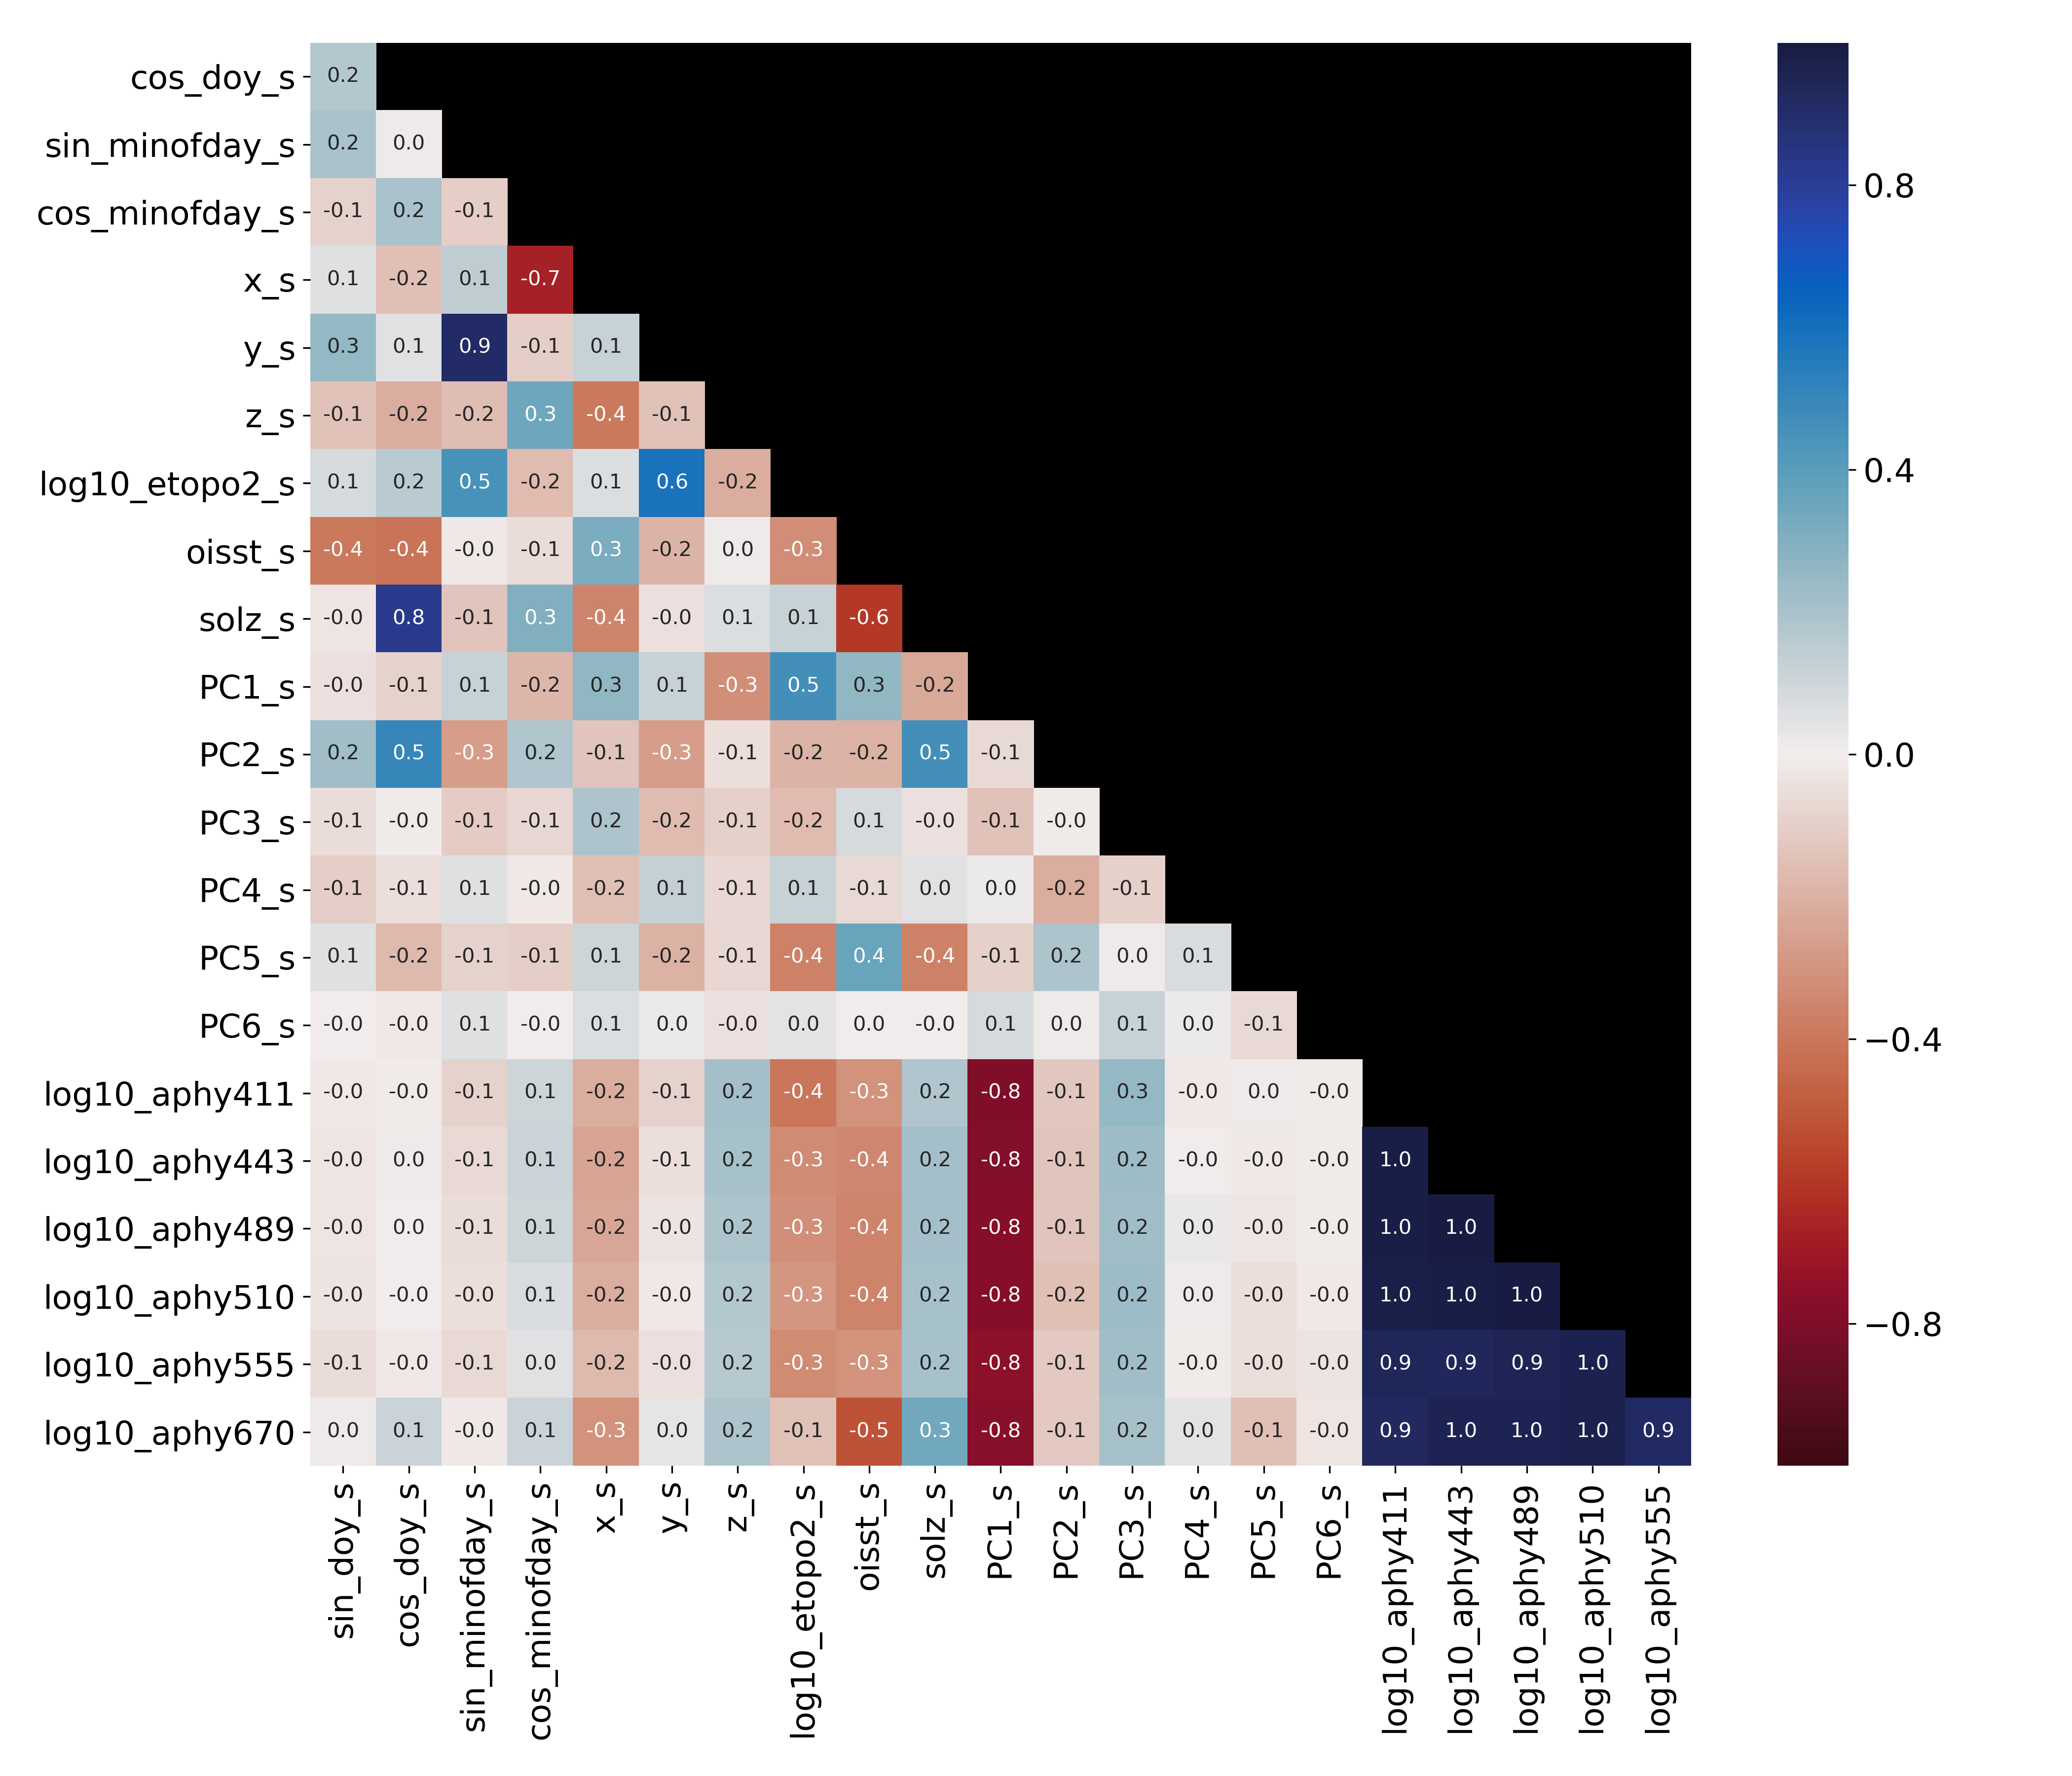
\includegraphics[scale=0.5]{feature_heatmap_annotated.png}
				\caption{Pairwise correlation plot of features and targets. Features are standardized; targets are log-transformed.}
			\end{figure}
		\subsection{Bayesian Neural Network Implementation}
			\subsubsection{Neural Networks and the Bayesian Paradigm}
				\begin{itemize}
					\item Neural Networks as function approximators
					\item Weights as distributions rather than scalar parameters
					\item Built-in regularization
					\item Out-of-the-box uncertainties
				\end{itemize}
			\subsubsection{Model Architecture and the Automatic Relevance Determination (ARD) Framework}
				\begin{itemize}
				    \item A bayesian hierarchical model is one in which the parameterization of coefficient distributions are dependent on an overarching distribution [include kruschke figure?]
				    \item A bayesian neural network with ARD is one where the variance of the distributions of the weights comming out of each input unit is controlled by a hierarchical distribution. This allows uncovering how relevant each feature is in predicting the target.
					\item Prior specification
				\end{itemize}
				\begin{figure}
				    \centering
				    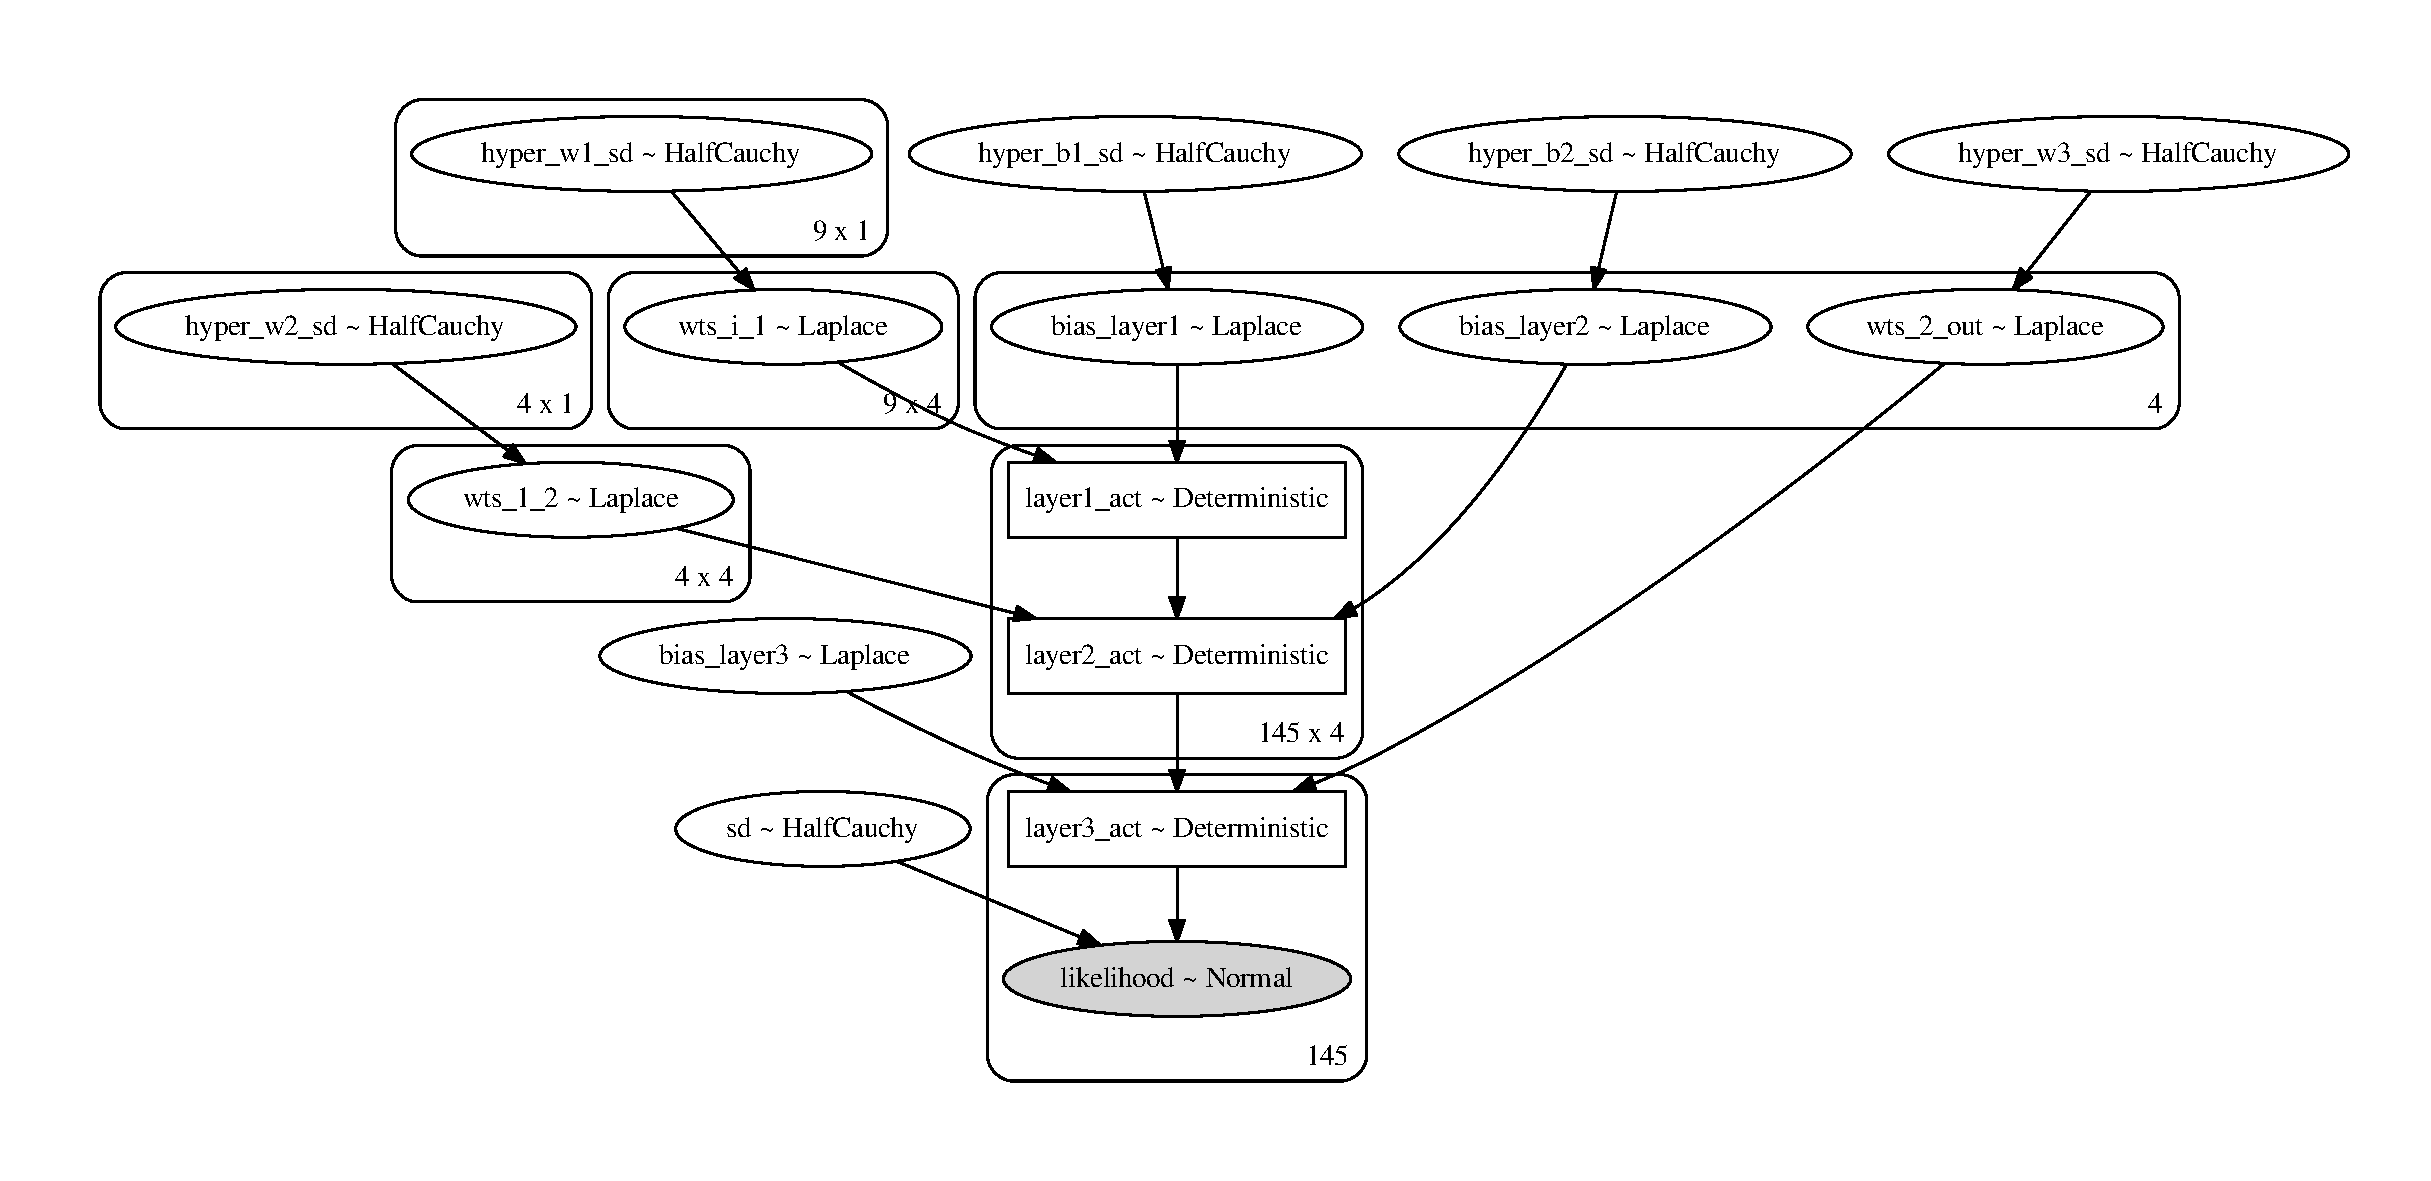
\includegraphics[scale=0.4]{bnn_l2_4_4_robust.pdf}
				    \caption{Bayesian Model Neural Network with two hidden layers of 4 units each, trained on 145 observations and 9 features. Each layer has also an additional bias unit. All weights and biases have Laplace (double-exponential) priors with scale parameterization drawn from Half-Cauchy hyperpriors. }
				\end{figure}
		\subsection{Data and Software Access, and Reproducibility}
		    \begin{itemize}
		        \item Code written in Python
		        \item Data preparation using pandas, numpy and scikit-learn
		        \item probabilistic programming in PyMC3
	            \item All code was written in python and is available as jupyter (formerly ipython) notebooks on github ($\rightarrow$ give reference). 
	            \item Data available on project repository, Open Science Framework ($\rightarrow$ give reference), and includes
	            \begin{itemize}
	                \item full and train/test-split dataset
	                \item Python standard scaler and PCA transformer objects parameterized for the data used here
	                \item PyMC3 models fitted to the data, as serialized Python objects stored in binary files.
    	        \end{itemize}
	       \end{itemize}
	\newpage
	\section{Results}
		\subsection{Model Comparison}
			\begin{itemize}
				\item WAIC
				\item LOOCV
			\end{itemize}
		\subsection{Test Set Validation And Posterior Predictive Checks}
			\begin{itemize}
				\item Test set observed/predicted comparison 
				\item Fig w/ r2 and mae
				\item Fig w/ 95\% and 50\% HPD]
			\end{itemize}
		\subsection{Posterior Distribution of Weights}
			\begin{itemize}
				\item Input unit weights posterior distribution in view of ARD
				\item Hidden unit weights posterior distribution
				\item Bias weights posterior distribution
			\end{itemize}
	\newpage
	\section{Discussion}
	\newpage
	\section{Conclusion}
	\newpage
	\section{References}
		\begin{itemize}
			\item McElreath Book
			\item Kruschke Puppy Book
			\item BDA 3
			\item PyMC3 paper
			\item Radford Neal's book on BNN
			\item SVGD paper
			\item McElreath Book chapter on WAIC
			\item LOOCV paper
			\item McKay on ARD
			\item Neal on ARD
		\end{itemize}
\end{document}